\documentclass{article}

% Submission: no options (anonymized, line numbers).
% Camera-ready: \usepackage[main, final]{neurips_2026}
% Preprint:     \usepackage[preprint]{neurips_2026}
\usepackage{neurips_2026}

\usepackage[utf8]{inputenc} % allow utf-8 input
\usepackage[T1]{fontenc}    % use 8-bit T1 fonts
\usepackage{hyperref}       % hyperlinks
\usepackage{url}            % simple URL typesetting
\usepackage{booktabs}       % professional-quality tables
\usepackage{amsfonts}       % blackboard math symbols
\usepackage{amsmath}        % equation environments (patched for line numbers)
\usepackage{graphicx}       % \includegraphics
\usepackage{nicefrac}       % compact symbols for 1/2, etc.
\usepackage{microtype}      % microtypography
\usepackage{xcolor}         % colors
\usepackage{amssymb}
\usepackage{tikz}
\usepackage{enumitem}
\usepackage{placeins}
\usetikzlibrary{arrows.meta,positioning}
\usepackage{svg}
\graphicspath{{../../figures/}}

\title{Activation Steering Corrupts Agent Beliefs}

\author{%
  Anonymous Author(s) \\
  Anonymous Affiliation \\
  \texttt{anonymous@example.com} \\
}

\begin{document}

\maketitle

\begin{abstract}
Activation steering is spreading from language models to Reinforcement Learning (RL) agents, where it is proposed as a lightweight test-time behavioral intervention. Whether such edits are safe for recurrent RL agents, which carry their beliefs in their hidden state is an open question. We introduce Cogniland, a procedurally generated partially observable navigation task in which an agent must integrate evidence into a belief about a hidden map property. We find that \textbf{(i)} the belief is encoded as a single direction of the recurrent state. one single scalar matches the performance as a non-linear probe on the full state \textbf{(ii)} such belief is causal: editing the hidden state along this direction gradually shifts the model’s decision on a downstream task. \textbf{(iii)} Steering the agent to suppress a navigation skill corrupts the belief and thus degrades the final decision performance. We attribute the corruption to entanglement: behavioral skills and belief states are not separable in hidden state. Steering methods for stateful agents need careful evaluation across different tasks and capabilities.
\end{abstract}

\section{Introduction}
What happens to an agent's belief when we steer its behavior? Activation
steering changes what a model does by adding a vector to its hidden
activations at inference time, with no retraining
\citep{turner2023actadd,rimsky2024caa,zou2023repe}. It is cheap, it needs only
a few contrasting examples, and it is being proposed as a safety tool. The
method is now moving from language models to reinforcement learning (RL)
agents, where it has been used to retarget a policy by editing its activations
\citep{mini2023maze}. Agents differ from language models in one way that
matters here: a recurrent agent in a partially observable world keeps its
belief about the hidden state of the world in the same hidden vector that the
steering edit modifies, and the recurrence carries the edit forward at every
step. An edit aimed at a behavior may therefore land on the belief as well.

The question is hard to answer in a language model, where beliefs have no
ground truth. We therefore build Cogniland, a procedurally generated navigation task
in which the belief is the hidden category of the map, the agent must
integrate evidence about it and carry it across a memory corridor, and its
skills, bridging water and tunnelling rock, can be counted. The belief shows
in the final decision, which of two flags the agent walks into, so belief and
behavior are measured separately, and the reward exposes a wrong belief on
some maps and hides it on others.

We train a recurrent PPO agent with no supervision on the category and study
its hidden state in three steps. First we decode the belief and find that it
is a single direction: a logistic regression on one scalar, the projection of
the state on the difference of class means, matches a non-linear probe on the
full state. Second we show that the direction is causal: one write along it
at the end of the corridor moves the flag decision with a sigmoidal dose
response, while random directions of the same size do nothing. Third we steer
a skill, suppressing bridging or tunnelling with gradient steps on the action
probability, and read the belief. The steering works as intended: the tool is
used less and the agent still reaches a flag on most maps. But when the
suppressed tool is the one the map's category needs, the belief moves toward
the other category and the agent walks to the wrong flag in most lakes
episodes and nearly half of the rocky ones (Figure~\ref{fig:illustration}).
Suppressing the other tool leaves the belief alone.

Side effects of steering have been reported in language models, where steering
vectors generalize unreliably \citep{tan2024reliability} and break safety
alignment \citep{korznikov2025rogue}. For agents that carry beliefs in a
recurrent state the question is almost unstudied. Our contributions are:
\begin{itemize}[leftmargin=1.4em, itemsep=1pt]
\item Cogniland, a partially observable navigation task with a ground-truth
belief and countable skills, and a recurrent agent that solves it from reward
alone.
\item The belief is one direction of the hidden state: a scalar reads it as
well as a non-linear probe, and writing to it controls the final decision
with a graded dose response.
\item Steering a navigation skill corrupts this belief and flips the final
decision while navigation stays mostly intact, a failure mode the return
cannot see on balanced maps.
\item We attribute the corruption to entanglement: behavior and belief are not
separable directions of the hidden state, so steering methods for stateful
agents should be evaluated across all capabilities, not only the targeted one.
\end{itemize}

\begin{figure}[htbp]

    \centering

    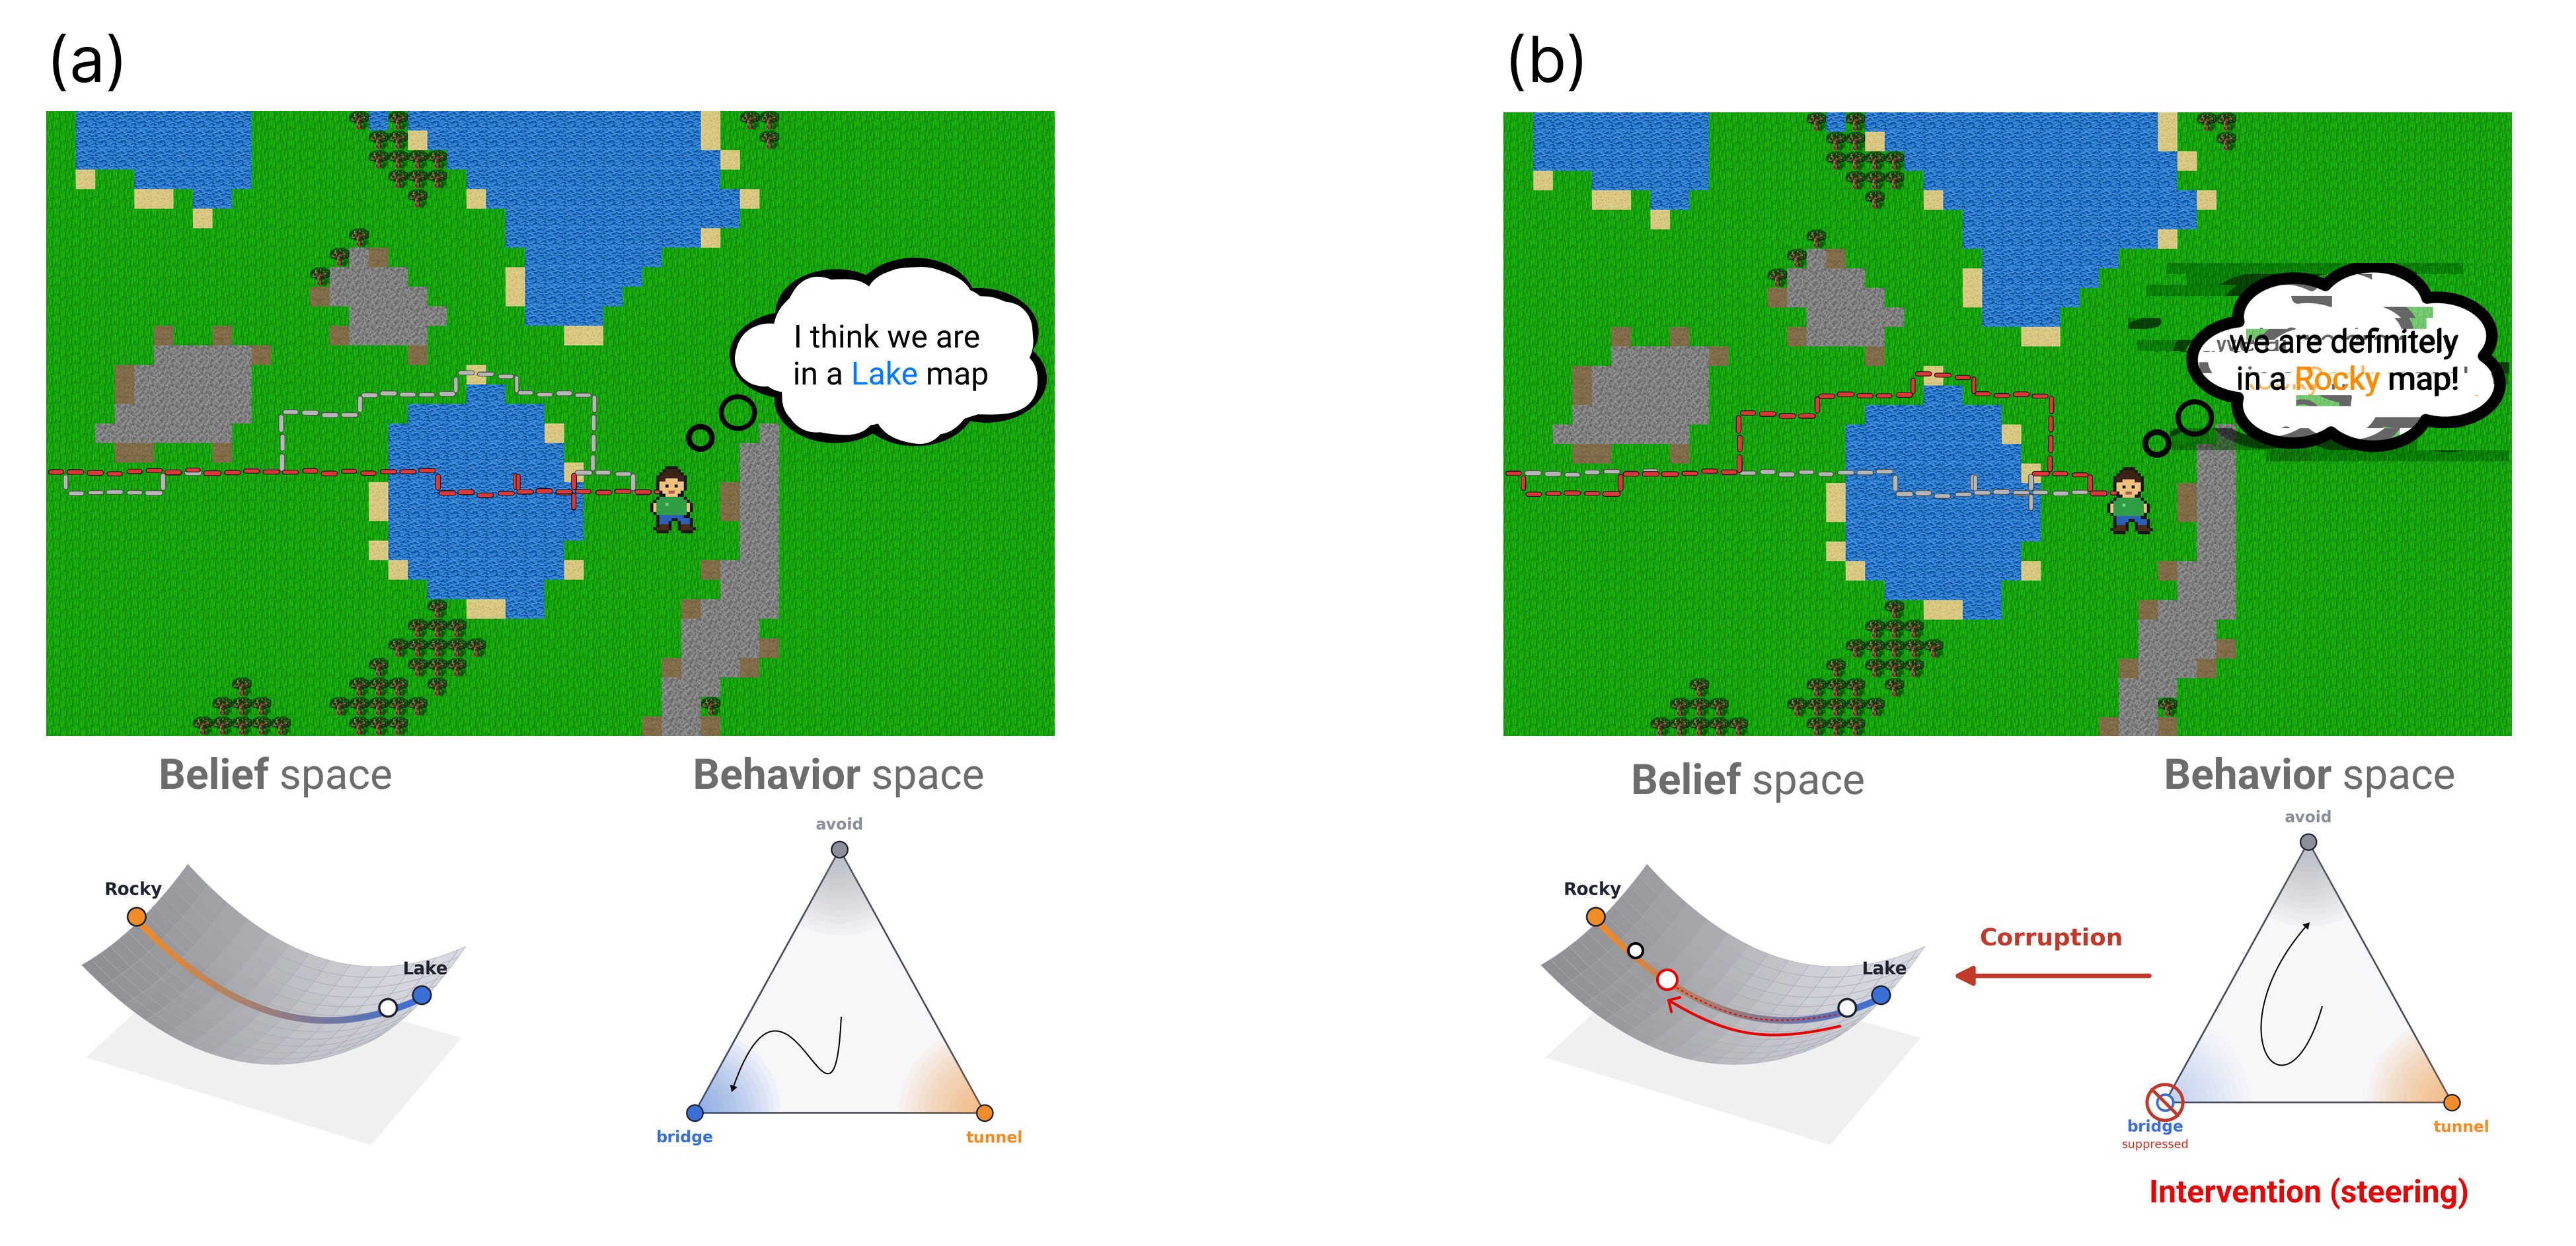
\includegraphics[width=0.95\linewidth]{figures/illustration.png}

    \caption{\textbf{Suppressing a skill corrupts the belief.} Two realizations of an agent deployed on a \textit{lakes} map (a) Unsteered agent: the agent crosses the water by building a bridge, and its belief correctly matches the real category (belief space). (b) Steered agent: bridging is suppressed by activation steering (behavior space): the route changes as intended, but the belief flips towards the wrong category.}
    \label{fig:illustration}

\end{figure}


% ---------------------------------------------------------------------------
% Method (concise). Details live in the appendix files sections/app_*.tex.
% Earlier versions: sections/method_prev*.tex.
% ---------------------------------------------------------------------------
\section{Methodology}
\label{sec:method}

\paragraph{Task.}
\label{sec:task}
Cogniland is a procedurally generated grid world built on OpenSimplex noise
\citep{spencer2014opensimplex}. A successful agent must develop navigation skills and belief integration ability. An episode is one $32\times64$ map crossed from
left to right (Figure~\ref{fig:task}, Appendix~\ref{app:map-generation}). Water
and rock tiles block movement and trees are impassable; the agent can \textsc{build} on the water and \textsc{mine} through rocks.
Each map has a hidden \emph{category} set by its terrain distribution:
\emph{lakes} (more water), \emph{rocky} (more rock) or \emph{balanced}. Every map ends in a narrow passage, followed by a split with two flags signaling terminal states. Only the correct flag pays a terminal reward: the top flag on rocky
maps, the bottom flag on lakes maps, either flag on balanced maps
(Appendix~\ref{app:map-generation}). The agent must form a \textbf{belief}
about the category and carry it across the grass corridor that precedes the passage, while using its
\textbf{skills} to get past the obstacles on the way. Map categories are sampled
uniformly during training.

\begin{figure}[h]
    \centering
    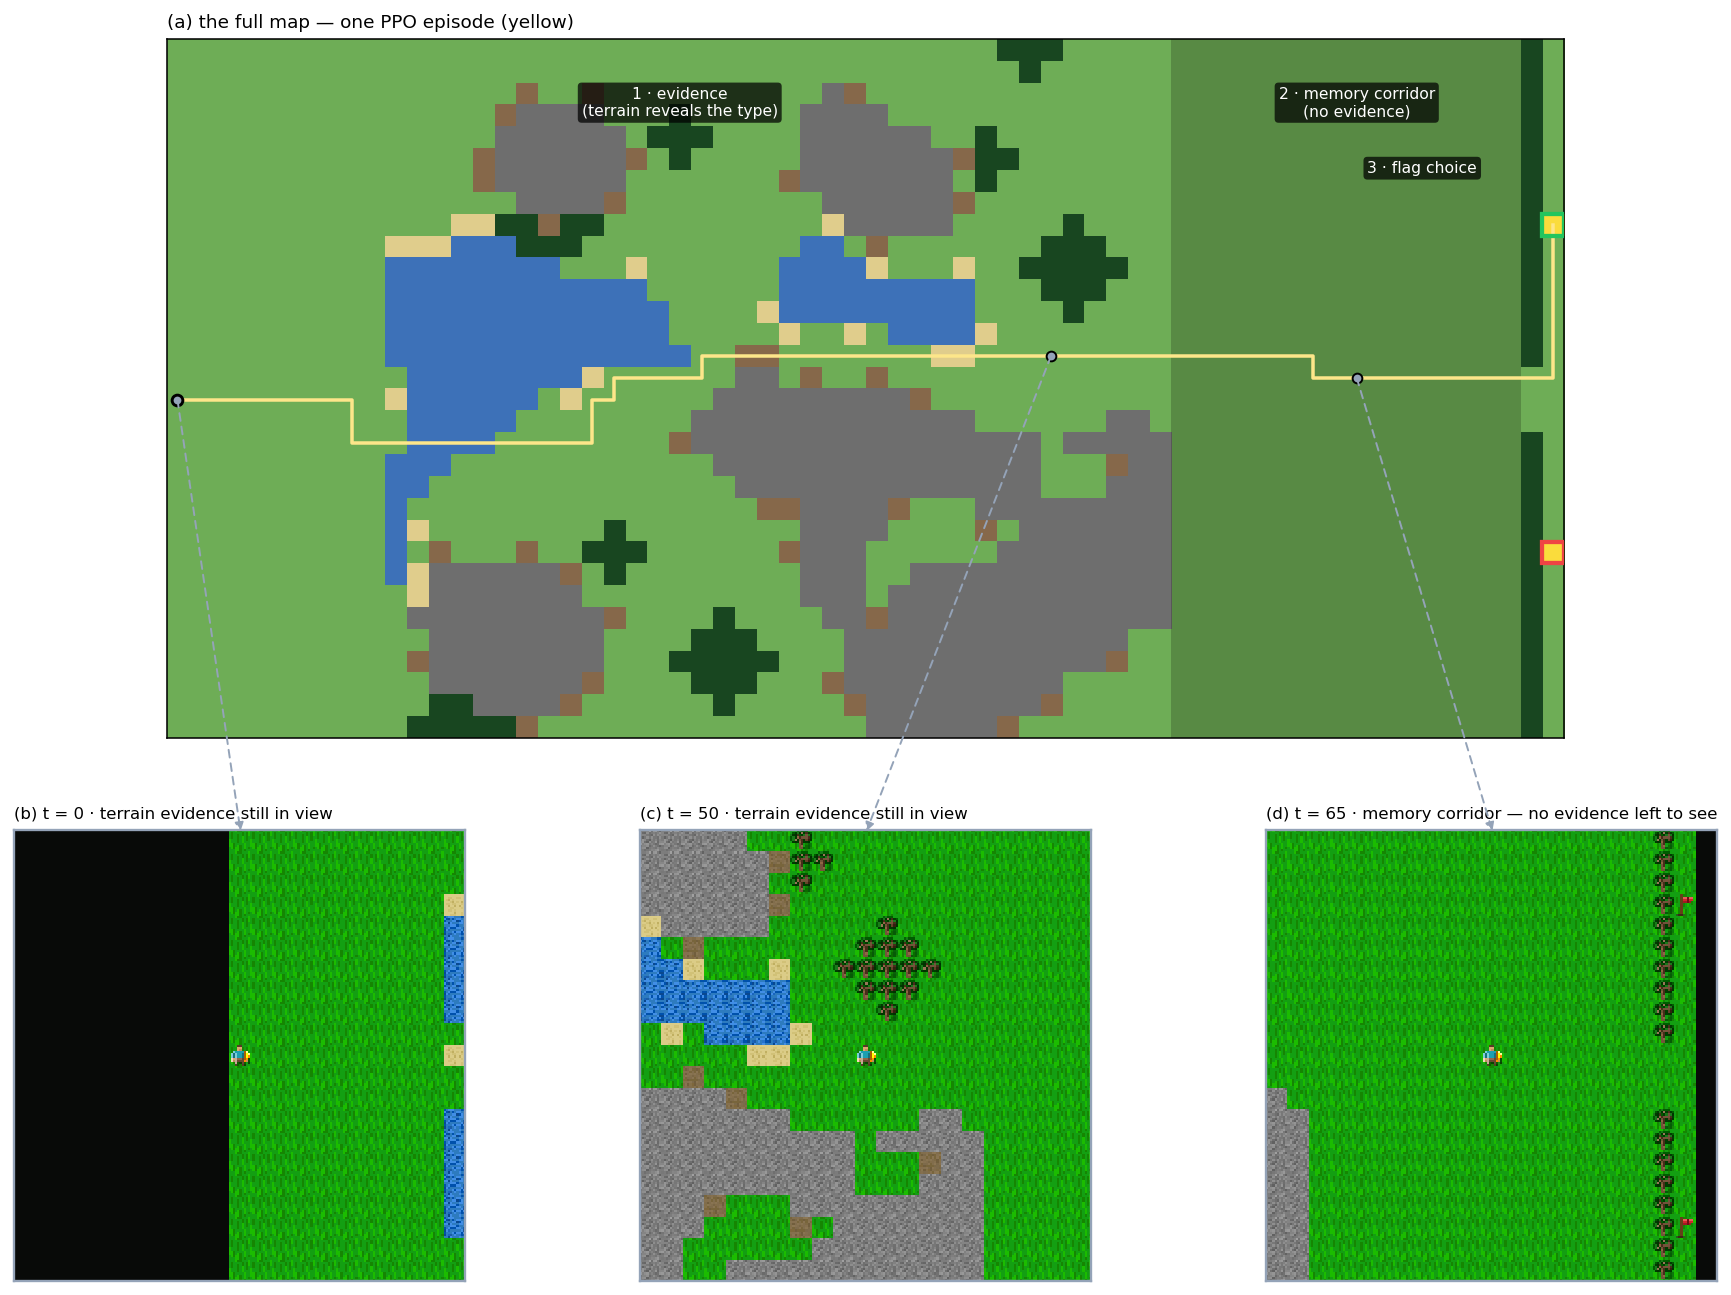
\includegraphics[width=0.6\linewidth]{figures/task.png}
    \caption{\textbf{Anatomy of an episode.} (a) an agent trajectory on a \textit{rocky} map (yellow). Bottom row shows $21\times21$ egocentric observations at different timesteps. (b) The agent starts with little evidence about the map. (c) During the episode the agent navigates obstacles and collects evidence about the map distribution. (d) The agent is presented a choice, only the correct flag returns terminal reward. The choice is determined by the acquired evidence over the episode.}
    \label{fig:task}
\end{figure}

\paragraph{Problem formulation.}
\label{sec:formulation}
The task is a Partially Observable Markov Decision Process (POMDP) with hidden
variable $c\in\{\text{lakes},\text{rocky},\text{balanced}\}$, observations
$o_t$ and actions $a_t$. Three quantities are defined per episode.
\emph{Belief:} $\beta_t = P(c\mid o_{1:t})$, the agent's estimate of which
kind of map it is on. A well-calibrated belief is necessary to achieve high reward: a
Bayes-optimal agent walks to the flag of the most probable category
$\arg\max_c \beta_t(c)$, and on balanced maps either flag is optimal.
The agent carries and updates its belief through the recurrent state
$\mathbf{h}_t$.
\emph{Behavior:} $\phi = (n_{\textsc{build}}, n_{\textsc{mine}})$, the
number of times the agent bridged water and tunnelled rock. Obstacles can be crossed with a tool or walked around (Appendix~\ref{app:measures}).
\emph{Decision:} $D\in\{\text{top},\text{bottom}\}$, the flag the agent
walks into. On lakes and rocky maps one flag pays nothing, so a wrong $D$
shows in the return; on balanced maps both pay, so $D$ is a free choice the
return cannot see.
A steering intervention $\mathcal{I}$ edits the hidden state $\mathbf{h}_t$ to
change the behavior $\phi$, for instance to suppress \textsc{mine} so that the
agent walks around mountains instead. Ideally the intervention $\mathcal{I}$ leaves the belief $\beta$,
and hence the final decision $D$, untouched. We measure \emph{belief corruption} as the change
in the decoded belief and in the final decision $D$ that $\mathcal{I}$ causes.

\paragraph{Model.}
\label{sec:model}
The agent is a recurrent actor-critic policy trained with PPO
\citep{schulman2017ppo} (Figure~\ref{fig:model}): a convolutional encoder of the egocentric view, with
coordinate channels appended \citep{liu2018intriguing}, feeds a GRU \citep{cho2014gru} with $128$-d hidden state $\mathbf{h}_t$. Linear actor
and critic heads read $\pi(a\mid\mathbf{h}_t)$ and the value $V(\mathbf{h}_t)$ from the hidden state. The
training loss is the PPO objective alone; nothing supervises $\mathbf{h}_t$ on
the category, so the belief we decode is emergent (Appendix~\ref{app:model}). Trained on $4{,}800$ maps, the best
agent reaches $98.8\%$ success evaluated on $1{,}200$ held-out maps.

\paragraph{Belief decoding.}
\label{sec:decoding}
Because the belief direction might change over the course of an episode, we split the map's columns into eight position bins, five over the evidence terrain, two over the memory corridor and one at the passage (Appendix~\ref{app:belief-causality}), and fit
and score every readout separately in each bin, evaluating on held-out maps.
In each bin we compare three readouts of $\mathbf{h}_t$: a logistic-regression probe, a one-hidden-layer MLP probe, and a logistic regression on a single scalar, the projection of $\mathbf{h}_t$ on the difference-of-means direction $\mathbf{v}$ between the activations of rocky and lakes maps over a bin. If the belief is linear and one-dimensional, the scalar should match the full-state probes' performance. An episode's belief $\hat b$ is the average projection $b_t=\mathbf{h}_t^{\top}\mathbf{v}$ over bin \textit{corr2}.

\paragraph{Belief causality.}
\label{sec:causality}
A direction may be decodable even if it is not used by the policy \citep{alain2017probes}. To test whether
$\mathbf{v}$ influences the flag decision, we push the state along this direction and leave every other
direction untouched,
$\mathbf{h}'=\mathbf{h}+s\,\alpha\,g\,\mathbf{v}$,
where $g=b^{\star}_{\text{rocky}}-b^{\star}_{\text{lakes}}$ is the distance between
the two category poles, $s=+1$ pushes toward rocky and $s=-1$ toward lakes, and
$\alpha$ is the dose: $\alpha=0$ is the unsteered agent and $\alpha=1$ moves the
belief coordinate by one full pole-to-pole distance. The write is applied once at
the entry of bin \textit{corr2}; lakes maps are pushed toward rocky, rocky maps
toward lakes and balanced maps in both directions, and the outcome is the
decision $D$ as a function of $\alpha$. As a control we apply a displacement of
the same size, $\alpha g$, along random directions.

\paragraph{Steering.}
\label{sec:steering}
Activation steering edits $\mathbf{h}_t$ directly, as popular steering methods
do \citep{turner2023actadd,rimsky2024caa,zou2023repe}. To suppress the skill
associated with an action $\bar a$, here \textsc{build} or \textsc{mine}, we
drive its probability $\pi(\bar a\mid\mathbf{h})$ below a threshold $\theta$ by
gradient steps in activation space:
\begin{equation}
\mathbf{h}\;\leftarrow\;\mathbf{h}-\alpha\,
\frac{\nabla_{\mathbf{h}}\log \pi(\bar a\mid\mathbf{h})}{\lVert\nabla_{\mathbf{h}}\log \pi(\bar a\mid\mathbf{h})\rVert}
\qquad\text{while } \pi(\bar a\mid\mathbf{h})>\theta.
\label{eq:clamp}
\end{equation}
This is applied at every step and carried forward by the recurrence. Steps already
below $\theta$ are left untouched, so $\theta$ sets the strength and $\alpha$
only the step size; a fixed steering vector is the unconditional, one-step
special case (Appendix~\ref{app:steering-algorithm}). Behavior change is the
reduction in successful uses of the suppressed tool relative to the unsteered
agent on the same maps and seeds. We measure the change in belief $\hat b$
and decision $D$ between the steered and unsteered realizations of the policy
(Appendix~\ref{app:measures}).


\section{Results}

\subsection{Belief is represented as a single direction}
\label{sec:res_belief}
Figure~\ref{fig:results_belief}a shows that accuracy rises with the evidence seen, from
$83\%$ in the first bin to $99\%$ from the corridor onwards: the decoded belief matches the real map category at every stage of the map. It is surprising that the non-linear MLP probe generalizes \emph{worse} than a single 1D logistic probe: it trails the scalar by nine points in the first bin and never leads it by more than one. All the information relevant for the belief lies along a single direction in activation space. This is what the linear representation hypothesis predicts \citep{park2024linear,elhage2022toy}: a network trained on a general loss represents each concept it learns as one direction in activation space.

This direction is not fixed across the stages of an episode. Figure~\ref{fig:results_belief}b shows that
neighbouring bins agree, with a cosine of $0.88$ between the two corridor bins, while the earliest and the last differ most with a similarity of $0.33$: it looks like the code drifts, perhaps as a rotation, as evidence accumulates over an episode. We therefore choose \textit{corr2} to fit the direction $\mathbf{v}$ where the belief is complete and the flags are not yet in view. Figure~\ref{fig:results_belief}c shows the logistic regression fit on $b_t=\mathbf{h}_t^{\top}\mathbf{v}$
achieving $\mathbf{98.9\%}$ accuracy on the $266$ lakes and rocky maps not used for the fit. $57\%$ of balanced maps,
never used to fit $\mathbf{v}$, are believed to be rocky while the remaining $43\%$ are more similar to lakes.

\begin{figure}[h!]
\centering
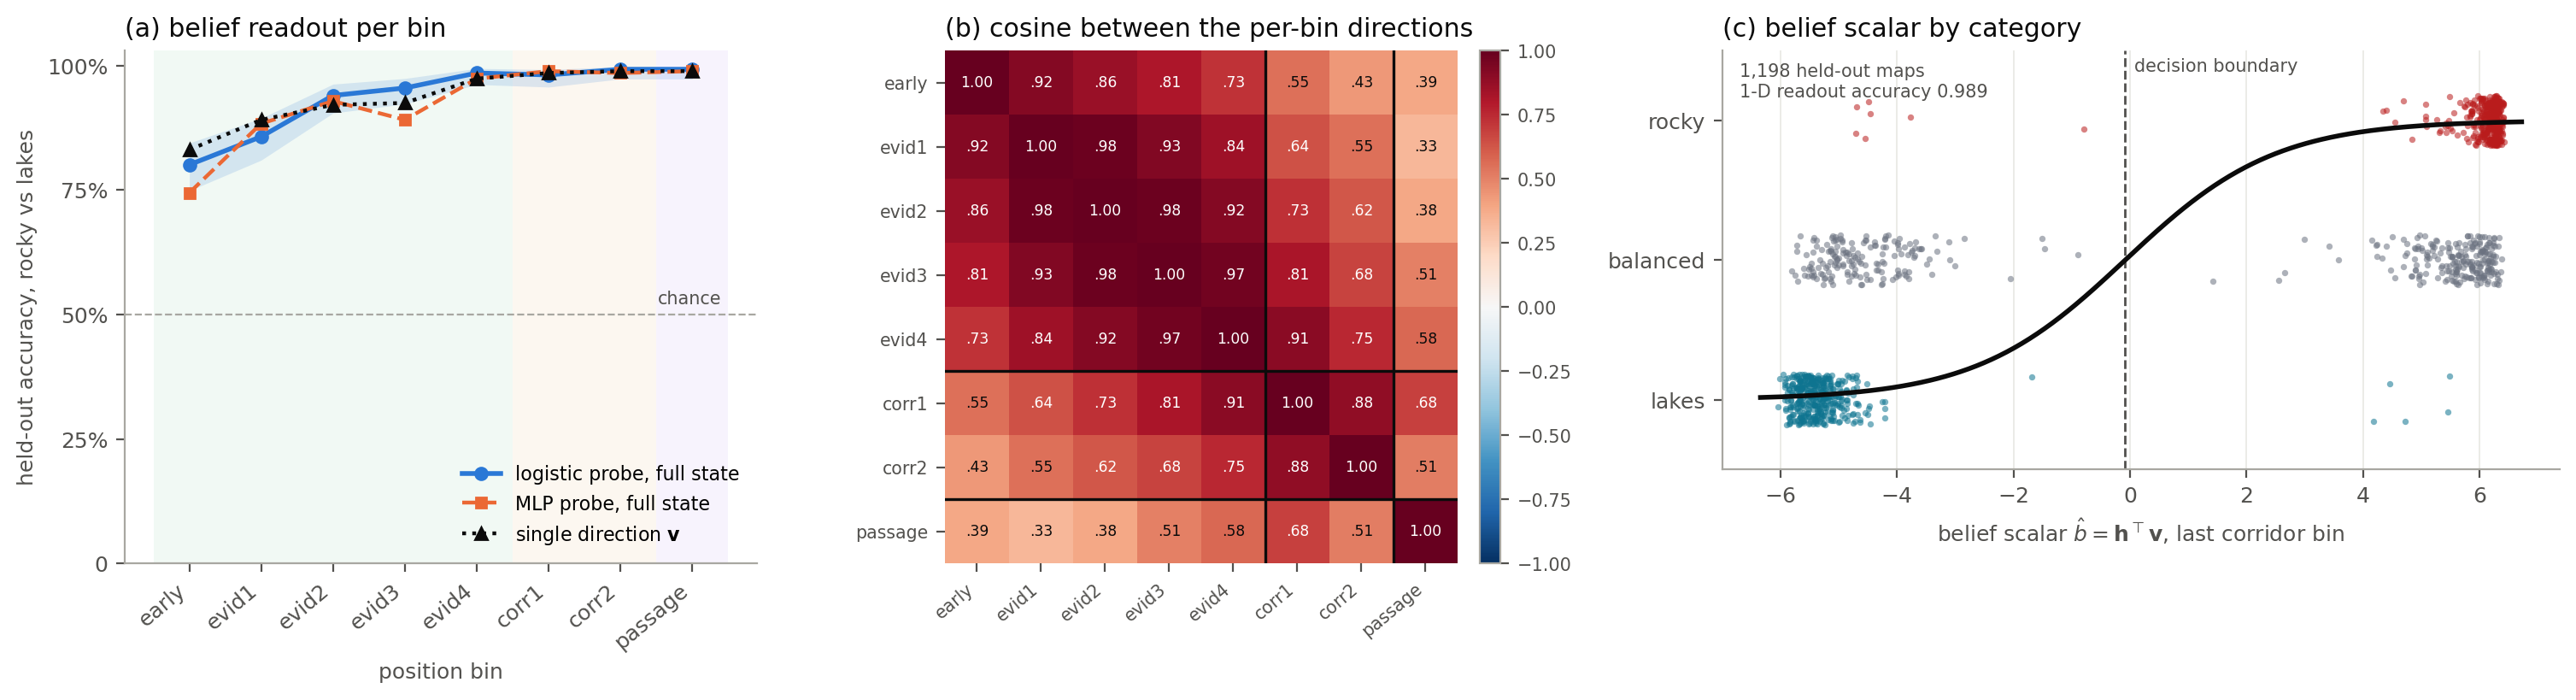
\includegraphics[width=\linewidth]{figures/fig_results_belief.png}
\caption{\textbf{Belief is represented as a single direction} (a) Held-out belief accuracy for rocky against lakes in every position
bin: (i) a logistic-regression probe and (ii) an MLP probe on the full $128$-d state,
and (iii) a logistic regression on the single scalar $b_t=\mathbf{h}_t^{\top}\mathbf{v}$,
where $\mathbf{v}$ is the difference-of-means direction. The scalar matches the full-state probes everywhere, and all three reach
$0.98$ or more from the corridor on. (b) Cosine between the directions $\mathbf{v}$ fitted in different bins.
(c) States projected on the belief direction per map category in bin \textit{corr2}; the curve is the logistic regression on this scalar, with $98.9\%$ held-out accuracy. $57\%$ of balanced maps are classified as rocky.}
\label{fig:results_belief}
\end{figure}

\subsection{The final decision depends on the belief}
\label{sec:res_causal}
Figure~\ref{fig:results_causal} shows which flag the agent chooses as a
function of the steering dose $\alpha$. Pushing the belief of a lakes map
toward rocky smoothly raises the probability of the top flag, until the agent
takes it every time; pushing a rocky map toward lakes does the mirror image.
The response is sigmoidal: small doses do nothing, then the decision flips
over a narrow range of $\alpha$, and by one pole-to-pole distance it has
saturated. On balanced maps, where the unsteered agent has a mild preference
for the top flag, the same write selects either flag on demand. The effect
belongs to the direction and not to the size of the edit: a displacement of
the same size along a random direction leaves the decision where the
unsteered agent put it. The write also costs nothing in navigation. Every
steered episode still reaches a flag, and the episodes are as long as the
unsteered ones. The belief direction is thus a clean handle on a high-level
decision: writing to it changes what the agent decides and nothing about how
it moves.

\begin{figure}[h!]
\centering

\includegraphics[width=0.7\linewidth]{figures/fig_results_causal.png}
\caption{\textbf{The belief direction moves the decision.} One write of
$\mathbf{h}\leftarrow\mathbf{h}\pm\alpha g\mathbf{v}$ at the entry of the last
corridor bin, where $\mathbf{v}$ is fitted, on $100$ held-out maps per
category for $\alpha\in\{0,0.1,\dots,1\}$; the flag taken is recorded, error
bars are one binomial standard deviation, $\alpha=0$ is the unsteered agent.
Lakes maps go from $2\%$ top flag to $100\%$ between $\alpha=0.4$ and $0.8$;
rocky maps from $100\%$ to $0$ between $0.5$ and $0.9$; balanced maps from
$62\%$ top to $100\%$ or to $0$ by $\alpha=0.9$. Dashed grey: the control, a
displacement of the same size $\alpha g$ along a random direction, stays
within $0.02$--$0.04$ on lakes, at $1.00$ on rocky and within $0.62$--$0.67$
on balanced maps. Every steered episode reaches a flag, and episode length
stays within three steps of the unsteered agent's at every dose.}
\label{fig:results_causal}
\end{figure}

\subsection{Behavioral steering corrupts the belief}
\label{sec:res_steer}
We steer the agent on the held-out maps where the unsteered agent uses both
tools at least once, six rollouts per map, and suppress one tool at a time
(Table~\ref{tab:clamp_all}). The behavior changes as intended: the suppressed
tool is used less on most maps, the other tool is barely affected, and the
agent still reaches a flag in nearly all episodes. Walking around a mountain
instead of tunnelling through it is costlier, so timeouts rise a little on
rocky maps, but navigation itself is intact. The intervention is a
gradient-based attack on the action distribution \citep{huang2017adversarial},
and at the action head it does exactly what it is asked.

It also does something it was not asked to do. Suppressing the tool that the
map's category needs moves the belief toward the other category, and the flag
decision follows. A lakes map on which the agent cannot bridge is read as a
rocky map: the belief readout crosses to the rocky side and most episodes end
at the rocky flag, which gives no reward. A rocky map on which the agent
cannot tunnel goes the same way in reverse, with the belief landing on the
boundary and almost half of the episodes at the lakes flag. On balanced maps,
where the reward cannot tell, the free choice is captured almost completely
by whichever tool is suppressed. The effect is one-directional: suppressing
the other tool, tunnelling on lakes maps or bridging on rocky maps, leaves
belief and flag where they were. An edit aimed at a skill lands on the
belief; the two are not separable directions of the hidden state.

\begin{table}[h!]
\centering
\small
\setlength{\tabcolsep}{6pt}
\caption{\textbf{Steering behavior corrupts the belief.} Gated gradient
steering on held-out maps where both tools are used at least once ($138$
balanced, $62$ lakes, $61$ rocky maps; six rollouts each). \emph{\# bridges}
and \emph{\# tunnels} are successful tool uses per episode, the lowest of
each category in bold; \emph{timeout} is the share of episodes that did not
reach a flag; \emph{rocky flag} and \emph{lakes flag} are the agent's
decision; $\hat b(\text{rocky})$ is the mean probability of the rocky category
read from the belief scalar by the logistic probe. Suppressing bridging on
lakes maps raises $\hat b(\text{rocky})$ from $0.03$ to $0.79$ and sends
$74\%$ of episodes to the rocky flag ($1\%$ unsteered); suppressing tunnelling
on rocky maps lowers it from $0.96$ to $0.50$ and sends $43\%$ to the lakes
flag ($4\%$ unsteered). Failure modes in red.}
\label{tab:clamp_all}
\begin{tabular}{@{}llrrrrrr@{}}
\toprule
& & & & \multicolumn{3}{c}{share of episodes} & \\
\cmidrule(lr){5-7}
Category & Regime & \# bridges & \# tunnels & timeout & rocky flag & lakes flag & $\hat b(\text{rocky})$ \\
\midrule
balanced & unsteered & 4.21 & 4.94 & 0.00 & 0.60 & 0.40 & 0.61 \\
 & suppress bridge & \textbf{2.61} & 4.79 & 0.01 & 0.97 & 0.02 & 0.97 \\
 & suppress tunnel & 4.12 & \textbf{3.83} & 0.06 & 0.19 & 0.75 & 0.23 \\
\midrule
lakes & unsteered & 6.04 & 1.92 & 0.00 & 0.01 & 0.99 & 0.03 \\
 & suppress bridge & \textbf{4.66} & 1.94 & 0.05 & \textcolor{red}{\textbf{0.74}} & 0.22 & 0.79 \\
 & suppress tunnel & 6.25 & \textbf{1.31} & 0.00 & 0.00 & 1.00 & 0.02 \\
\midrule
rocky & unsteered & 1.98 & 6.86 & 0.00 & 0.96 & 0.04 & 0.96 \\
 & suppress bridge & \textbf{0.96} & 7.03 & 0.00 & 1.00 & 0.00 & 0.99 \\
 & suppress tunnel & 2.02 & \textbf{5.42} & 0.14 & 0.43 & \textcolor{red}{\textbf{0.43}} & 0.50 \\
\bottomrule
\end{tabular}
\end{table}



\section{Related work}
% Activation Steering Compromises LLM Safety https://arxiv.org/abs/2509.22067
% Steering Vectors are an Adversarial Attack Surface https://arxiv.org/abs/2606.05958


\section{Discussion}
We proposed an environment where the agent integrates the belief of hidden variable while navigating obstacles in a complex naturalistic map generated through OpenSimplex noise. We applied activation steering on a recurrent RL agent and found that steering navigation skills corrupts the agent's linear belief, showcasing a failure mode. Steering methods for stateful agents should be judged across all capabilities, not only on the targeted behavior.

\subsection{Limitations}
All results come from one agent, one architecture and one task trained with PPO. We don't know whether belief and skills are entangled in the same way in larger recurrent networks, in transformer policies or in world-model agents.
We test one family of interventions, gradient steps on the action probability. Finally, we infer
entanglement from the direction of the leak; we do not explain why the gradient of the action head has a component along the belief direction.

\subsection{Future directions}
The first question is whether a steering method can leave the belief untouched. Two options are to project the steering step onto the directions orthogonal to the belief, or to steer a model-based agent through imagination \citep{hafner2023dreamerv3}. The same question applies to language models and to vision-language-action (VLA) models, whose activations also carry beliefs about the user, the task and the scene that steering may corrupt in the same way. Cogniland gives ground-truth beliefs for this test. Extending
this to richer beliefs, longer episodes, and a broader range of skills could provide further insights into the relationship between cognitive and motor tasks in AI agents.


\bibliographystyle{plainnat}
\bibliography{references}

\appendix
APPENDIX NOT REVIEWED

\section{Measures and statistics}
\label{app:measures}
\paragraph{Behaviour.}
Behaviour is counted in \emph{successful} tool events, a rock actually removed
or a plank actually placed, never in action presses, which repeat when the
agent is blocked. On the held-out balanced maps used for steering, a
tool-free route to a flag exists on every map (cost-to-go reachability with
both tools disabled), so suppressing a tool never makes a map unsolvable,
only costlier. Every steered episode is paired with the unsteered agent on
the same map and the same rollout seed; we report the per-map percentage
change in the suppressed tool, summarised as the median over maps and the
number of maps on which the count fell, together with the untouched tool's
count. Task outcome is the true flag metric, whether the final cell is a
rewarding flag, never a positive return, since a fast wrong-flag episode
collects more shaping than it loses in slack. Failures are split into timeouts
and wrong flags; on balanced maps we also record the top-flag rate.

\paragraph{Belief corruption.}
The belief shift of an episode is $\Delta\hat b=\hat b_{\text{steered}}-\hat b_{\text{unsteered}}$, paired per map. Its scale is set by a \emph{seed-only
null}, the unsteered agent re-run with fresh rollout seeds on the same maps,
whose per-map $|\Delta\hat b|$ is the noise floor, so shifts are reported in
floors. We also report the crossing rate, the fraction of steered episodes
whose belief crosses the midpoint $m$, and the per-map shift of the chosen
flag against the same null. A \emph{null edit} sets $\theta=1$, a threshold that can
never be exceeded, so the clamp never fires and the trajectory is
byte-identical to the unsteered one. A \emph{matched random
direction} re-runs every episode applying the per-step displacement
magnitudes recorded from the real edit along directions that carry no
information, redrawn at every step or drawn once and held for the episode.
Significance is a paired sign-flip permutation test over maps with $20{,}000$
draws, and every quantity reported as within its floor comes with a
percentile bootstrap interval over maps.

\FloatBarrier

\section{Procedural generation of maps}
\label{app:map-generation}
\paragraph{Observations, actions, reward.}
The observation is an egocentric $21\times21$ crop of the tile map, one-hot
over nine tile types, plus five scalars: the facing direction as a one-hot of
four and the elapsed fraction of the step budget. The action space is
\texttt{Discrete(6)}: four moves, \textsc{build} and \textsc{mine}. The reward
is
\begin{equation}
r_t \;=\; -0.01 \;+\; 0.015\,(d_{t-1}-d_t) \;+\; 3\cdot\mathbf{1}[\text{correct flag}],
\label{eq:reward}
\end{equation}
where $d_t$ is the cost-to-go in cells to the nearest rewarding flag. The
middle term is potential-based shaping \citep{ng1999shaping} in its
undiscounted form, so pacing back and forth nets nothing. Episodes end at any
flag or after $800$ steps; the discount is $\gamma=0.99$.

\paragraph{Generation, step by step.}
Every map is a deterministic function of an integer seed and a category.
Figure~\ref{fig:mapgen} shows the six stages on one real map; the parameters
are collected in Table~\ref{tab:mapgen}.
\begin{enumerate}[leftmargin=1.4em, itemsep=1pt]
\item \textbf{Heightmap.} A five-octave OpenSimplex field
\citep{spencer2014opensimplex} on the $32\times64$ grid, octave $k$ at
wavelength $\lambda_0/2^k$ with weight $2^{-k}$, normalised by the weight sum.
\item \textbf{Domain warp.} Two independent two-octave fields displace the
sampling coordinates by up to $0.10\max(H,W)$ cells, so lakes and massifs get
irregular coastlines instead of blobs.
\item \textbf{Overlays.} Two to four lakes are carved and two to four
mountains raised, each a round logistic disk or an irregular massif of three to
five Gaussian lobes with equal probability, and at most one meandering ridge is
added. Radii are drawn small-biased, $R = \max(H,W)\,(0.02 + 0.075\,u^2)$ with
$u\sim\mathcal{U}(0,1)$.
\item \textbf{Quantile threshold.} Cells below the $w$-quantile of the field
become water and cells above the $(1-r)$-quantile become rock, so every map hits
its category's water and rock fractions $(w,r)$ exactly: lakes $(0.245,
0.035)$, rocky $(0.035, 0.245)$, balanced $(0.14, 0.14)$. Sand and dirt
speckles are added on a fraction of the one-cell ring around water and rock;
both are walkable and only cosmetic.
\item \textbf{Bands, trees, corridor.} The ten leftmost and rightmost columns
are cleared; the agent spawns at the middle of the left edge. About $3\%$ of
cells become impassable tree patches of radius one or two, placed with a strong
bias toward the top and bottom rows so that hugging the top or bottom edge is not a free route;
patches are removed, last placed first, until the flags are reachable with
trees as the only barrier. The sixteen columns before the passage are then reset
to grass: the memory corridor.
\item \textbf{Passage and flags.} A line of trees one column from the right
edge, open only at a three-cell passage at the middle rows, and two single-cell flags on the right
edge at one quarter and three quarters of the height. The rewarding flag is the
bottom one when $w > 1.5\,r$, the top one when $r > 1.5\,w$, and either
otherwise.
\item \textbf{Winnability guard.} A breadth-first search from the spawn to the
rewarding flag treating the category's crossable tile as passable (water for
lakes, rock for rocky, each in turn for balanced) must succeed; otherwise the
seed is advanced by a large prime and the map regenerated, up to $400$ times.
\end{enumerate}

\begin{figure}[t]
\centering
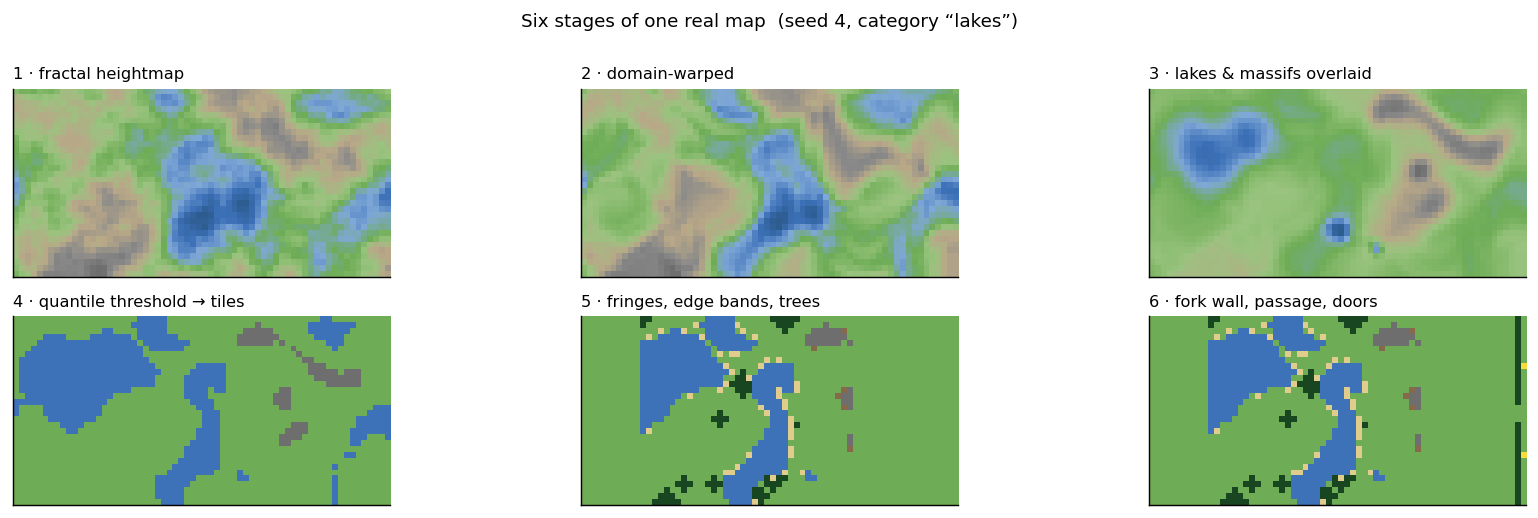
\includegraphics[width=\linewidth]{figures/mapgen_pipeline.png}
\caption{\textbf{One map, six stages.} Fractal heightmap, domain warp, overlaid
lakes and massifs, quantile threshold to tiles, cosmetic fringes with edge bands
and tree patches, and finally the passage and flags. The example is a
lakes map; a rocky map differs only in the two quantiles of step~4.}
\label{fig:mapgen}
\end{figure}

\begin{table}[t]
\centering
\footnotesize
\caption{\textbf{Map-generation parameters.} $H\times W = 32\times64$;
$\max(H,W)=64$. Uniform integer ranges are inclusive.}
\label{tab:mapgen}
\begin{tabular}{@{}p{3.0cm}p{4.5cm}p{5.5cm}@{}}
\toprule
Parameter & Value & Meaning \\
\midrule
Base wavelength $\lambda_0$ & $\max(H,W)/4.5 = 14.2$ cells & largest terrain feature of the noise \\
Octaves & $5$: $\lambda_0/2^k$, weight $2^{-k}$ & fractal sum, $k=0,\dots,4$ \\
Warp fields & $2$ octaves ($\lambda_0$, $\lambda_0/2$; weights $1$, $0.5$) & one field per axis, independent seeds \\
Warp amplitude & $0.10\max(H,W) = 6.4$ cells & maximum coordinate displacement \\
Lakes / mountains & $2$--$4$ each & carved ($-1.3f$) / raised ($+1.3f$) \\
Feature shape & disk or massif, $p=0.5$ & disk: logistic edge, softness $\max(1.5, 0.3R)$; massif: $3$--$5$ lobes, $\sigma=0.6R$ \\
Feature radius $R$ & $64\,(0.02+0.075u^2)$, $u\sim\mathcal{U}(0,1)$ & $1.3$--$6.1$ cells, small-biased \\
Ridges & $0$--$1$ & capsule, length $0.15$--$0.32\cdot64$, width $0.03$--$0.045\cdot64$, wiggle $0.06\cdot64$, period $0.45\cdot64$ \\
Water / rock quantiles & $w$ / $1-r$ per category & lakes $(0.245, 0.035)$, rocky $(0.035, 0.245)$, balanced $(0.14, 0.14)$ \\
Sand / dirt speckle & $30\%$ / $25\%$ of the one-cell ring & cosmetic, walkable \\
Edge bands & $10$ columns, left and right & obstacle-free \\
Tree fraction & $0.03$ ($\approx 61$ cells) & patches of radius $1$--$2$, edge-biased rows \\
Memory corridor & $16$ columns before the passage & grass only \\
Passage, flags & column $62$, rows $15$--$17$; rows $8$ and $23$ of column $63$ & three-cell gap in a line of trees; two single-cell flags \\
Resampling & seed $+\,100003$, up to $400$ times & until the winnability guard passes \\
\bottomrule
\end{tabular}
\end{table}

\paragraph{Dataset.}
Seeds are drawn from disjoint blocks per category ($0$, $10^7$ and
$2\cdot10^7$ plus the map index), $2{,}000$ maps per category. Within each
category the maps are shuffled with a fixed seed and split $80/20$, giving
$4{,}800$ training and $1{,}200$ held-out maps, $400$ per category in the test
set. The agent is trained on the training pool only. Every measurement in this
paper is made on held-out maps, and every knob is chosen on training maps and
frozen before a held-out map is seen.
Figure~\ref{fig:dataset} shows five held-out maps of each category.

\begin{figure}[t]
\centering
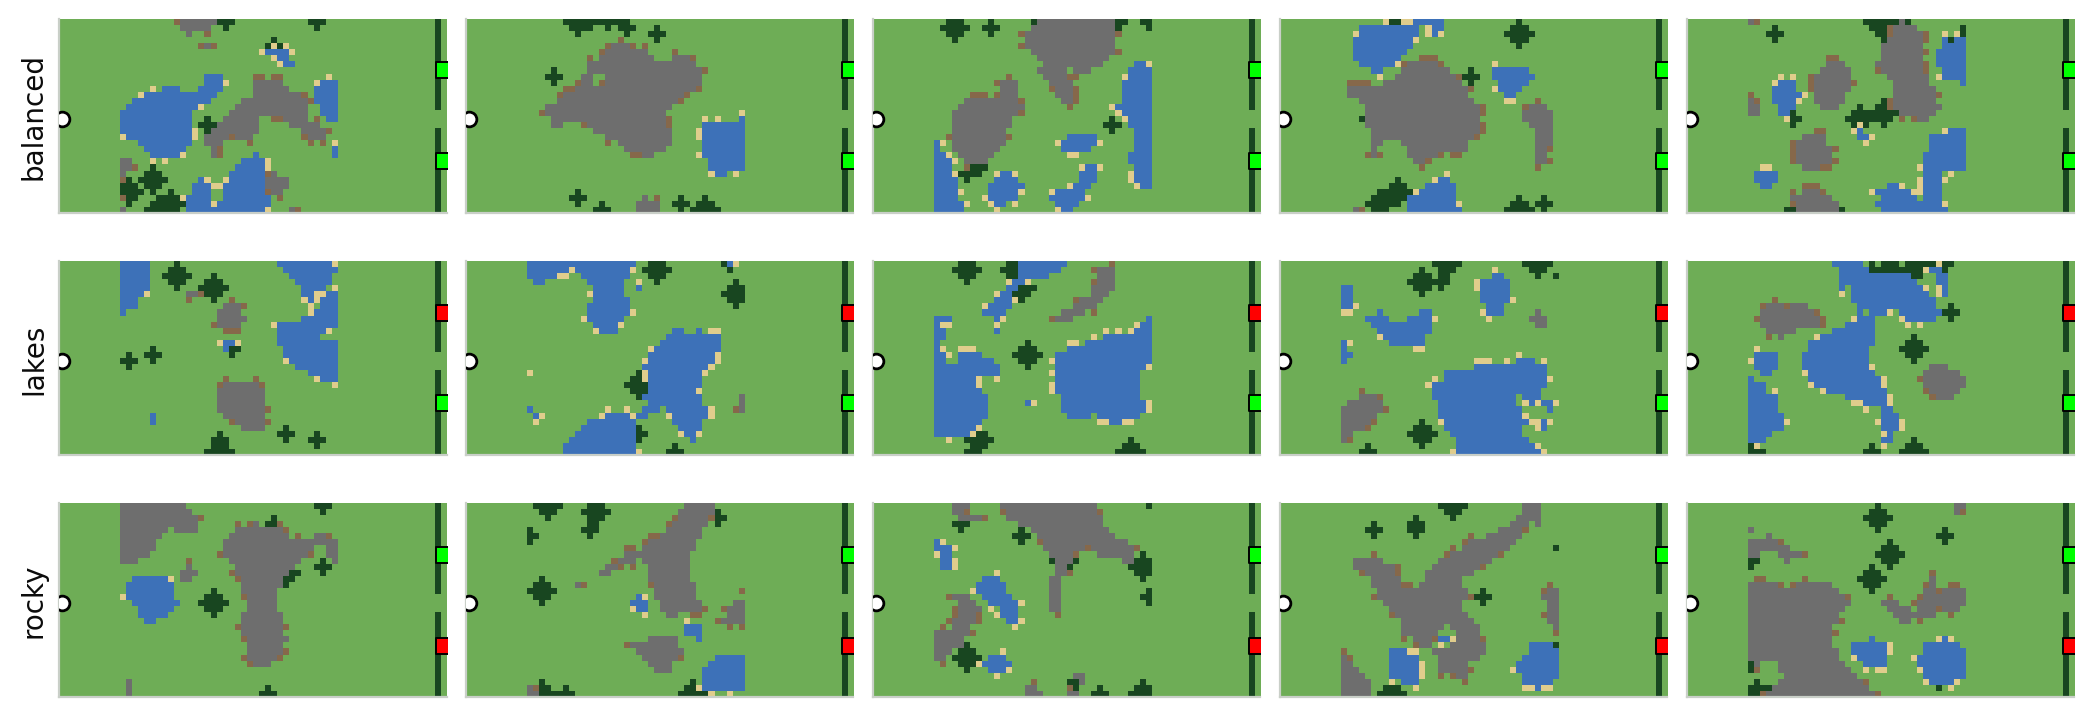
\includegraphics[width=\linewidth]{figures/fig_dataset_maps.png}
\caption{\textbf{Held-out maps by category}, five per row. Rows: balanced,
lakes, rocky. The white dot is the spawn, the green square the rewarding flag
and the red square the flag that pays nothing; on balanced maps both are
green. The three categories share one generator and differ only in the water
and rock quantiles, so no single tile identifies the category: it must be
integrated from the terrain seen along the way.}
\label{fig:dataset}
\end{figure}

\FloatBarrier

\section{Model, training and the feed-forward control}
\label{app:model}

\paragraph{Architecture.}


Table~\ref{tab:arch} lists the network layer by layer. The tile crop is one-hot
over nine tile types with two coordinate channels appended, the CoordConv
construction of \citet{liu2018intriguing}; three valid $3\times3$
convolutions reduce it to $15\times15\times32$, the flattened features and the
five scalars are projected to a $256$-d embedding, and a single-layer GRU with a
$128$-d state carries the only memory. Two linear heads read the state. There is
no other head and no other loss: the map category is never given to the network
as a target, so any belief in $\mathbf{h}_t$ is learned from reward alone.

\begin{figure}[h]
    \centering
    % PPO+GRU agent. Included from sections/method.tex.
\resizebox{\linewidth}{!}{%
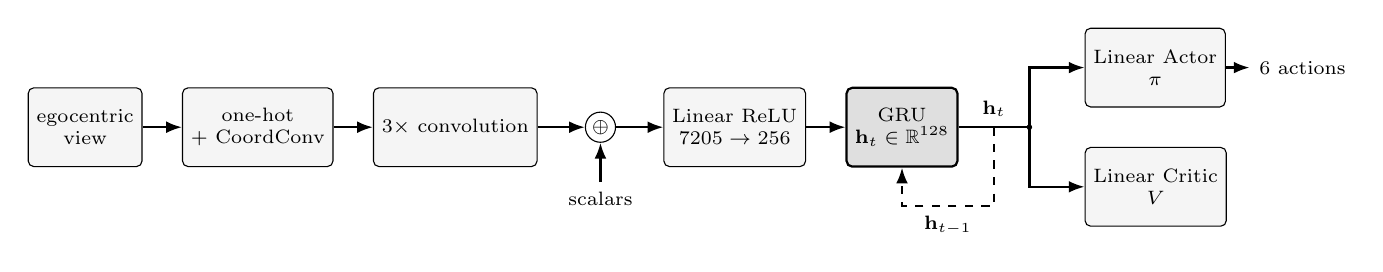
\begin{tikzpicture}[
  font=\scriptsize,
  box/.style={draw, rounded corners=2pt, fill=gray!8, minimum height=10mm,
              inner sep=3pt, align=center},
  arr/.style={-{Latex[length=2mm]}, thick},
  node distance=5mm and 5mm]
  \node[box] (obs) {egocentric\\view};
  \node[box, right=of obs] (enc) {one-hot\\$+$ CoordConv};
  \node[box, right=of enc] (cnn) {$3\times$ convolution};
  \node[circle, draw, inner sep=1pt, right=6mm of cnn] (cat) {$\oplus$};
  \node[box, right=6mm of cat] (mlp) {Linear ReLU\\$7205\to256$};
  \node[box, right=of mlp, fill=gray!25, thick] (gru) {GRU\\$\mathbf{h}_t\in\mathbb{R}^{128}$};
  \node[below=5mm of cat] (sc) {scalars};
  \coordinate[right=9mm of gru] (split);
  \node[box, above right=2.5mm and 7mm of split] (actor) {Linear Actor\\$\pi$};
  \node[box, below right=2.5mm and 7mm of split] (critic) {Linear Critic\\$V$};
  \node[right=3mm of actor] (acts) {$6$ actions};
  \draw[arr] (obs) -- (enc);
  \draw[arr] (enc) -- (cnn);
  \draw[arr] (cnn) -- (cat);
  \draw[arr] (cat) -- (mlp);
  \draw[arr] (sc) -- (cat);
  \draw[arr] (mlp) -- (gru);
  \draw[thick] (gru) -- (split) node[midway, above] {$\mathbf{h}_t$};
  \draw[arr] (split) |- (actor);
  \draw[arr] (split) |- (critic);
  \draw[arr] (actor) -- (acts);
  \fill (split) circle (1pt);
  \draw[arr, dashed] (split) ++(-4.5mm,0) -- ++(0,-10mm) -| (gru.south)
        node[pos=0.25, below] {$\mathbf{h}_{t-1}$};
\end{tikzpicture}}
\caption{\textbf{The agent.} The $21\times21$ tile view is one-hot encoded with
    two coordinate channels appended \citep{liu2018intriguing}, passed through
    three layers of convolutions, concatenated with five scalars (the facing direction as a one-hot of four and the elapsed time).
    This vector is projected to a
    $256$-d embedding, which is fed to a GRU with $128$-d hidden state $\mathbf{h}_t$. The actor and critic are linear projections of $\mathbf{h}_t$.}
    \label{fig:model}
\end{figure}
\begin{table}[h]
\centering
\small
\caption{\textbf{Architecture of the PPO+GRU agent.} The two coordinate
channels follow \citet{liu2018intriguing}. Weights are initialised
orthogonally, the actor with gain $0.01$. $2{,}015{,}559$ parameters in total.}
\label{tab:arch}
\begin{tabular}{@{}llrr@{}}
\toprule
Layer & Detail & Output & Parameters \\
\midrule
Input & $21\times21$ crop, one-hot $9$ tiles $+\,2$ CoordConv channels & $21\times21\times11$ & -- \\
Conv 1 & $3\times3$, valid, ReLU & $19\times19\times32$ & $3{,}200$ \\
Conv 2 & $3\times3$, valid, ReLU & $17\times17\times32$ & $9{,}248$ \\
Conv 3 & $3\times3$, valid, ReLU & $15\times15\times32$ & $9{,}248$ \\
Embedding & flatten $(7{,}200)$ $\oplus$ $5$ scalars $\to$ linear, ReLU & $256$ & $1{,}844{,}736$ \\
GRU & single layer, state $\mathbf{h}_t$ & $128$ & $148{,}224$ \\
Actor & linear, categorical over $6$ actions & $6$ & $774$ \\
Critic & linear & $1$ & $129$ \\
\bottomrule
\end{tabular}
\end{table}

\paragraph{Training.}
Table~\ref{tab:hparams} gives every hyperparameter. The loss is the clipped
PPO objective with a value term and an entropy bonus \citep{schulman2017ppo},
advantages from generalised advantage estimation \citep{schulman2016gae}, and
backpropagation through time over each $128$-step rollout. The entropy
coefficient starts at $0.15$ and is annealed linearly to zero. This schedule is
what makes the plain reward solvable: with a small entropy bonus the policy
settles on a constant flag, which already pays on two thirds of maps, and
never learns to use the category. The released agent is the best of five
belief-free seeds at entropy $0.15$; four solved the task and one collapsed
to the constant flag (Figure~\ref{fig:training}, Table~\ref{tab:seeds}). Runs at entropy $0.10$ and $0.20$ also solved the
task, so the recipe is not fragile in that knob. An otherwise equal agent
trained with an auxiliary category head scores the same held out, so
supervising the belief buys nothing.

\begin{figure}[h]
\centering

\includegraphics[width=\linewidth]{figures/training_curves.png}
\caption{\textbf{Training curves, mean $\pm$ one standard deviation over five
seeds.} Return per episode, success on all maps, and success on the decisive
lakes and rocky maps, against environment steps. The feed-forward control
plateaus at the constant-flag optimum: two thirds of maps overall and chance
on the decisive ones. The recurrent agent's band is wide early and late
because one of its five seeds collapses to the same constant flag; the others
reach near-perfect success.}
\label{fig:training}
\end{figure}

\begin{table}[h]
\centering
\small
\caption{\textbf{Training hyperparameters.} Identical for the recurrent agent
and the feed-forward control.}
\label{tab:hparams}
\begin{tabular}{@{}lr@{}}
\toprule
Hyperparameter & Value \\
\midrule
Environment steps & $6\times10^6$ \\
Parallel environments $\times$ rollout length & $32\times128$ \\
Minibatches per update $\times$ epochs & $4\times4$ \\
Optimiser, learning rate & Adam, $3\times10^{-4}$, constant \\
Discount $\gamma$, GAE $\lambda$ & $0.99$, $0.95$ \\
Clip $\epsilon$ & $0.2$ \\
Value coefficient & $0.5$ \\
Entropy coefficient & $0.15 \to 0$, linear over training \\
Gradient-norm clip & $0.5$ \\
Observation encoding & one-hot tiles, $21\times21$ view \\
Map pool & $4{,}800$ training maps, categories sampled uniformly \\
Evaluation & sampled actions, $1{,}200$ held-out maps \\
\bottomrule
\end{tabular}
\end{table}

\paragraph{Compute.}
Each run used one NVIDIA RTX~3090 of a shared SLURM cluster, with the $32$
environments stepped on the CPU, at about $2{,}450$ environment steps per
second for the recurrent agent and $8{,}000$ for the feed-forward control:
roughly $40$ minutes for a recurrent run and $13$ minutes for a feed-forward
run of $6$\,M steps. The whole sweep of twelve runs fits in a few GPU-hours.

\paragraph{Feed-forward control.}
To separate navigation from memory we train the same network with the GRU
replaced by a per-step linear layer with ReLU of the same width, so the agent
sees exactly the same input and has exactly the same heads but no carried
state. Five seeds with the same schedule as the recurrent agent, $6$\,M steps
each; all converge within the first million steps (Figure~\ref{fig:training}). Table~\ref{tab:seeds} gives the held-out result
of every seed of both agents. The feed-forward agent learns navigation: it
reaches a flag on every map and crosses water and rock as needed. What it
cannot do is choose the flag: each seed settles on one constant flag, so it is
right on all balanced maps and on one of the two decisive categories, at
chance on the decisive maps as a whole. The gap between the two agents is
therefore the memory itself, the belief integrated across the corridor.

\begin{table}[h]
\centering
\small
\caption{\textbf{Held-out results of every seed}, $1{,}200$ test maps, one
sampled rollout per map; both agents trained for $6$\,M steps with identical
hyperparameters. \emph{Decisive} is success on lakes and rocky maps,
where chance is $50\%$; \emph{top} is the share of balanced maps exited by the
top flag. Every feed-forward seed reaches a flag on essentially every map but
always the same one, so it scores $100\%$ on balanced maps, $100\%$ on one
decisive category and $0\%$ on the other. Four of five recurrent seeds solve
the task; seed~1 fell into the same constant-flag optimum. $^\dagger$The
released agent. Evaluations sample actions, so repeated runs of one checkpoint
differ by a few tenths of a point.}
\label{tab:seeds}
\begin{tabular}{@{}lrrrrrr@{}}
\toprule
& Overall & Decisive & Balanced & Lakes & Rocky & Top (balanced) \\
\midrule
\multicolumn{7}{@{}l}{\emph{GRU (recurrent)}} \\
seed 1 & 66.4 & 49.8 & 99.8 & 99.5 & 0.0 & 0.0 \\
seed 2$^\dagger$ & 98.8 & 98.2 & 100.0 & 98.5 & 98.0 & 57.2 \\
seed 3 & 97.8 & 97.0 & 99.2 & 94.2 & 99.8 & 64.0 \\
seed 4 & 98.5 & 97.8 & 100.0 & 97.5 & 98.0 & 41.2 \\
seed 5 & 97.2 & 96.1 & 99.5 & 98.2 & 94.0 & 71.0 \\
mean $\pm$ std & 91.8 $\pm$ 12.7 & 87.8 $\pm$ 19.0 & 99.7 $\pm$ 0.3 & 97.6 $\pm$ 1.8 & 78.0 $\pm$ 39.0 & 46.7 $\pm$ 25.3 \\
\addlinespace
\multicolumn{7}{@{}l}{\emph{Feed-forward control}} \\
seed 1 & 66.5 & 49.9 & 99.8 & 99.8 & 0.0 & 0.0 \\
seed 2 & 66.5 & 49.9 & 99.8 & 0.0 & 99.8 & 99.8 \\
seed 3 & 66.2 & 49.9 & 99.0 & 0.0 & 99.8 & 99.0 \\
seed 4 & 66.5 & 49.9 & 99.8 & 0.0 & 99.8 & 99.8 \\
seed 5 & 66.4 & 49.8 & 99.8 & 0.0 & 99.5 & 99.8 \\
mean $\pm$ std & 66.4 $\pm$ 0.1 & 49.9 $\pm$ 0.1 & 99.6 $\pm$ 0.3 & 19.9 $\pm$ 39.9 & 79.8 $\pm$ 39.9 & 79.7 $\pm$ 39.8 \\
\bottomrule
\end{tabular}
\end{table}




\FloatBarrier

\section{Activation dataset}
\label{app:dataset}
All belief analyses run on one activation dataset: the released agent plays
each of the $1{,}200$ held-out maps exactly once with sampled actions, and
every timestep is recorded. Episodes are seeded as $1000 + \text{map id}$, and
a replay under the same seed reproduces the stored trajectory action for action,
which is what lets a steered re-run be diffed against its baseline step by
step. The PPO half holds $106{,}473$ steps. Per step we store the $128$-d GRU
state the actor consumed (float16, $27$\,MB) and the variables of
Table~\ref{tab:steps}; per episode, the summary of Table~\ref{tab:episodes}.
The same protocol was recorded for two world-model agents on the same maps and
seeds; this paper uses only the PPO agent.

\begin{table}[t]
\centering
\small
\caption{\textbf{Variables logged at every timestep.} Positions are grid
coordinates with the origin at the top-left corner. ``Seen'' counts are taken
at first sight: a cell contributes once, when it first enters the $21\times21$
view.}
\label{tab:steps}
\begin{tabular}{@{}lp{9.6cm}@{}}
\toprule
Variable & Description \\
\midrule
\texttt{ep}, \texttt{map\_id} & Episode index and index of the map in the held-out pool (equal, one episode per map) \\
\texttt{category} & The map's hidden category: lakes, rocky or balanced \\
\texttt{t} & Timestep within the episode \\
\texttt{row}, \texttt{col} & Agent position before acting \\
\texttt{facing} & Facing direction (up, down, left, right) \\
\texttt{action} & Action taken: four moves, \textsc{build}, \textsc{mine} \\
\texttt{reward} & Reward received for this step (Equation~\ref{eq:reward}) \\
\texttt{ret} & Cumulative return up to and including this step \\
\texttt{water\_seen}, \texttt{rock\_seen} & Cumulative number of water and rock cells seen so far, the evidence available to the agent \\
\texttt{water\_now}, \texttt{rock\_now} & Number of water and rock cells in the current view \\
\texttt{phase} & \emph{evidence} (before the corridor), \emph{corridor}, or \emph{past\_wall} (at or beyond the passage) \\
\texttt{col\_rel\_wall} & Column relative to the passage (negative before it); the time axis of every binned analysis \\
$\mathbf{h}_t$ & The GRU state that produced the action, stored separately as a $128$-d vector \\
\bottomrule
\end{tabular}
\end{table}

\begin{table}[t]
\centering
\small
\caption{\textbf{Variables logged per episode.}}
\label{tab:episodes}
\begin{tabular}{@{}lp{9.6cm}@{}}
\toprule
Variable & Description \\
\midrule
\texttt{correct\_target} & The rewarding flag: top, bottom or either \\
\texttt{seed} & Rollout seed, $1000 + \texttt{map\_id}$ \\
\texttt{steps} & Episode length \\
\texttt{success} & Whether the final cell is a rewarding flag (the true flag metric) \\
\texttt{door} & Flag entered: top, bottom or none (timeout) \\
\texttt{final\_row}, \texttt{final\_col} & Final position \\
\texttt{ret} & Episode return \\
\texttt{builds}, \texttt{mines} & Successful bridge placements and rock removals, the behaviour counts $\phi$ \\
\texttt{water\_seen}, \texttt{rock\_seen} & Total water and rock cells seen over the episode \\
\bottomrule
\end{tabular}
\end{table}

\FloatBarrier

\section{Belief linearity}
\label{app:belief-causality}
\paragraph{Probes.}
We index time by the agent's column relative to the passage and bin it into an
evidence phase, a corridor phase and the passage. On states $\mathbf{h}_t$
collected from held-out maps, split by map into $801$ maps for fitting and
$399$ for testing, we train a logistic-regression probe and a one-hidden-layer
MLP probe to predict the three-way category at each bin, against a
shuffled-label null. The gap between the two probes measures how non-linear
the code is.

\paragraph{The single direction.}
Let $\mu_{\mathrm r}$ and $\mu_{\mathrm l}$ be the means of $\mathbf{h}_t$ over
the eight columns immediately before the passage on rocky and lakes training
maps; $\mathbf{v}=(\mu_{\mathrm r}-\mu_{\mathrm l})/\lVert\mu_{\mathrm r}-\mu_{\mathrm l}\rVert$.
An episode's belief $\hat b$ is $b_t=\mathbf{h}_t^{\top}\mathbf{v}$ averaged
over the same eight columns before the first passage crossing; the class means
of $\hat b$ are the category poles $b^{\star}_{\text{rocky}}$ and $b^{\star}_{\text{lakes}}$
and their midpoint $m$ the decision boundary, and an
episode has \emph{crossed} when $\hat b$ lies on the other side of $m$ from its
unsteered value. To price the reduction from $128$ dimensions to one we fit a
logistic regression on $\hat b$ alone and one on the full state under
five-fold cross-validation over training maps, refitting $\mathbf{v}$ inside
each fold so the whole pipeline is scored. Balanced maps are never used to fit
$\mathbf{v}$.

\paragraph{Causal test.}
We write to the coordinate and leave every other direction untouched,
\begin{equation}
\mathbf{h}' \;=\; \mathbf{h} + \big(b_{\lambda} - \mathbf{h}^{\top}\mathbf{v}\big)\,\mathbf{v},
\qquad
b_{\lambda} \;=\; (1-\lambda)\,b^{\star}_{\text{own}} + \lambda\,b^{\star}_{\text{other}},
\label{eq:set}
\end{equation}
where $b^{\star}_{\text{own}}$ is the pole of the map's true category,
$b^{\star}_{\text{other}}$ that of the other labelled category, and $\lambda$
the dose: $\lambda=0$ writes the agent's own category, a null write that
should change nothing, and $\lambda=1$ writes the opposite category. The write is applied once at corridor entry
(transient) or at every step from entry (sustained). The outcome is the flag
taken; on balanced maps we set $b_{\lambda}$ to each category's pole and report the top-flag rate.
The control writes the same displacement $\lVert\mathbf{h}'-\mathbf{h}\rVert$
along random unit directions on the same maps with the same timing.

\paragraph{Position bins and the geometry of the belief.}
All per-bin analyses use the eight bins of Figure~\ref{fig:bins}: five over the
evidence terrain, two over the memory corridor, and one at the passage.
Figure~\ref{fig:pca} projects the per-map bin means of lakes and rocky maps on
the first two principal components of those states, with the per-bin
difference-of-means direction drawn as a segment between the two class means.
Figure~\ref{fig:pca_balanced} shows each category separately in that plane with its per-bin mean.

\begin{figure}[t]
\centering
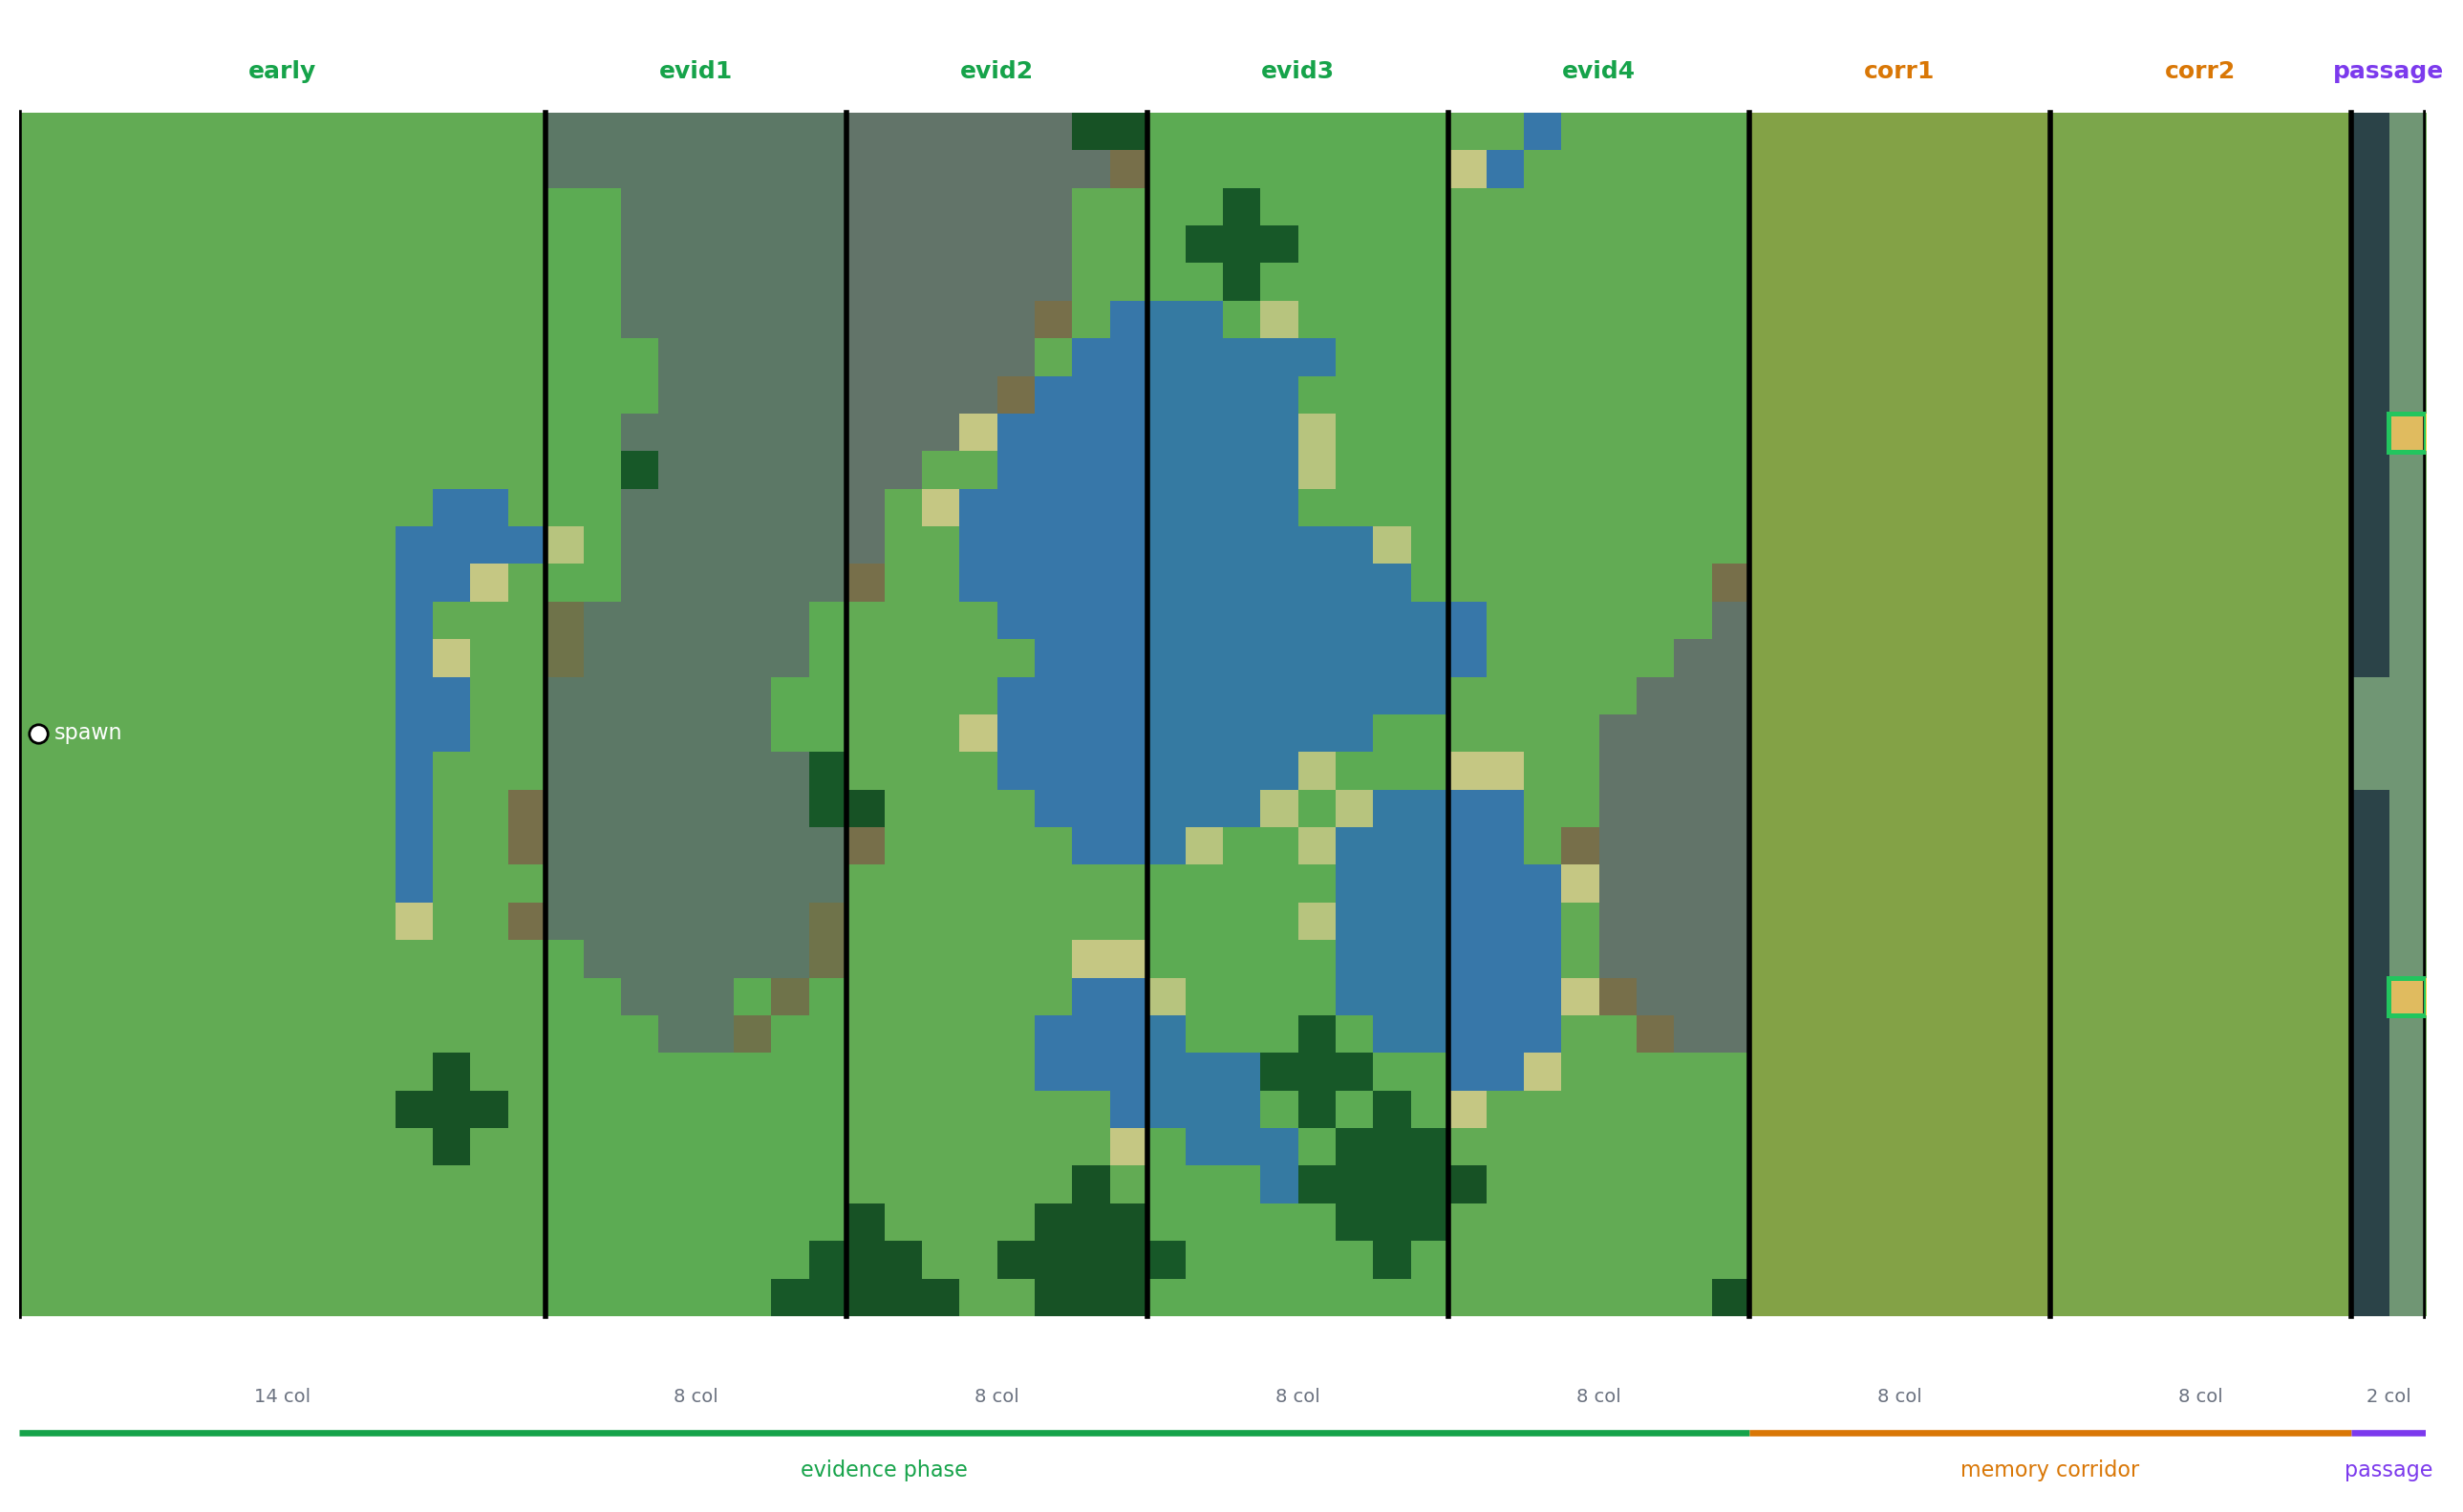
\includegraphics[width=\linewidth]{figures/fig_bins.png}
\caption{\textbf{The eight position bins}, drawn on a held-out balanced map.
Episodes are aligned by the agent's column relative to the passage rather than
by time, so agents of different speeds are compared at the same place. Five
bins cover the evidence terrain, two the memory corridor, and one the passage.}
\label{fig:bins}
\end{figure}

\begin{figure}[t]
\centering
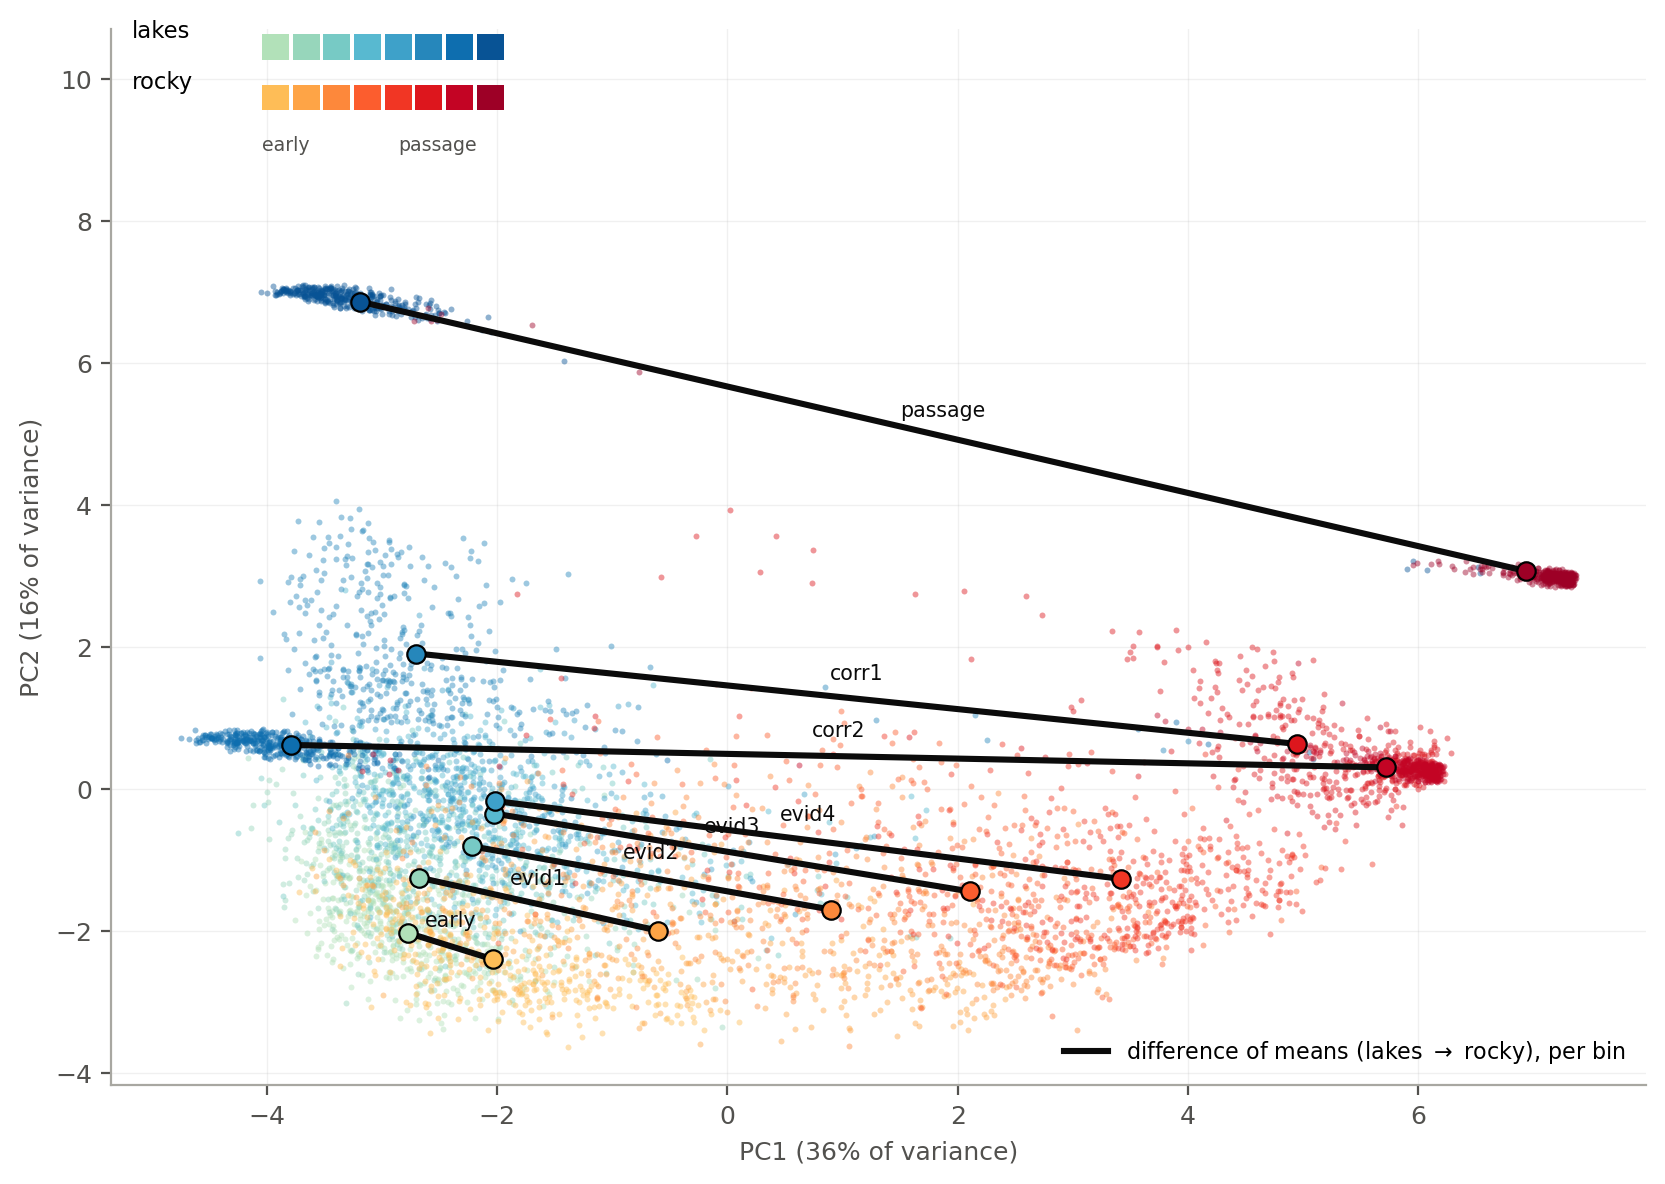
\includegraphics[width=0.9\linewidth]{figures/fig_pca_lakes_rocky.png}
\caption{\textbf{Lakes and rocky states in the first two principal
components.} One point per map and bin, hue for the category and lightness for
the bin; segments join the lakes and rocky class means of each bin, i.e.\ the
per-bin single direction. PC1 seems to encode the rocky belief: rocky states
move steadily to the right as evidence accumulates and pin at the far right by
the passage. PC2 seems to encode the lakes belief: lakes states stay left and
rise sharply in the corridor and at the passage. The two categories therefore
separate along different axes late in the episode, and the difference-of-means
direction rotates accordingly.}
\label{fig:pca}
\end{figure}

\begin{figure}[t]
\centering
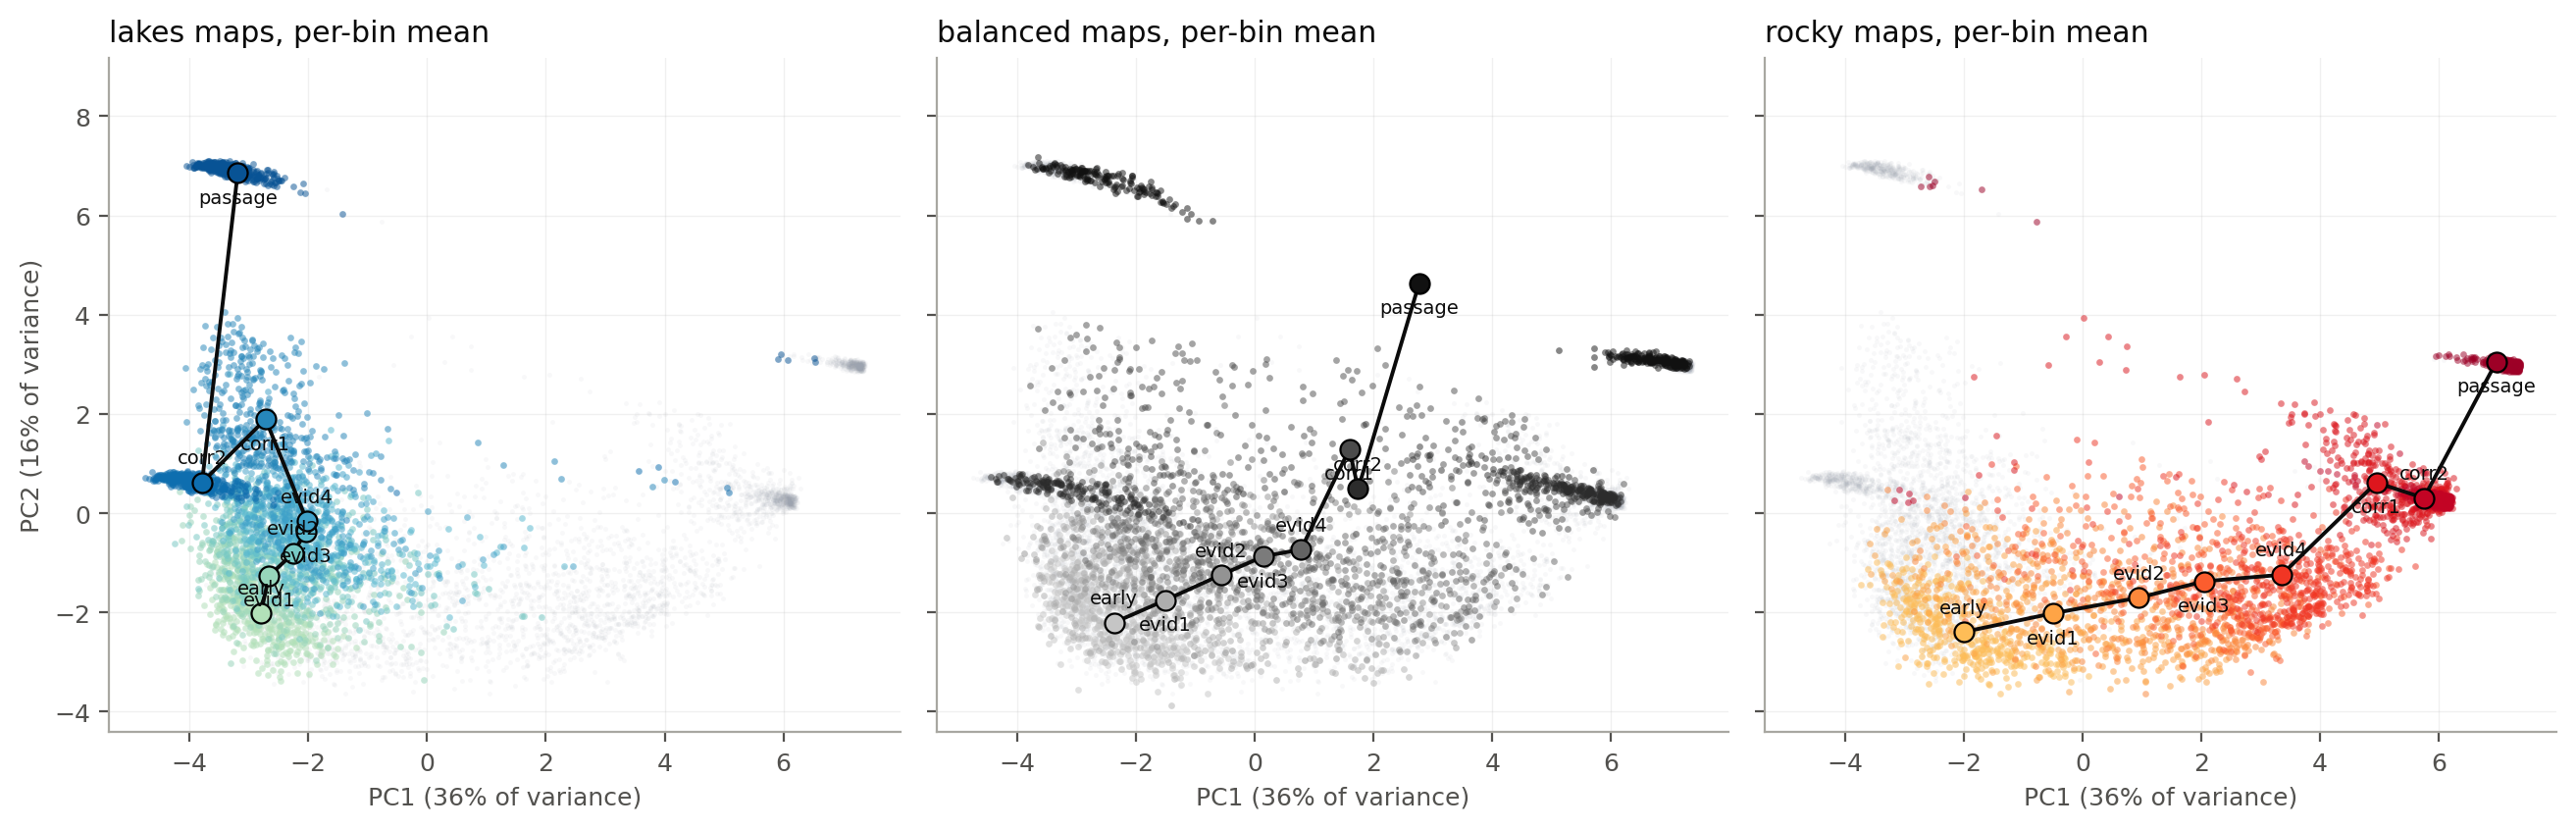
\includegraphics[width=\linewidth]{figures/fig_pca_categories.png}
\caption{\textbf{Each category in the same plane, with its per-bin mean.} The
plane is the one of Figure~\ref{fig:pca}, fitted on lakes and rocky states;
the full lakes-and-rocky cloud is drawn faintly in every panel for reference,
points are shaded by bin and the black path joins the per-bin means. Lakes
maps stay left and rise sharply in the corridor and at the passage. Balanced
maps, never used to fit the plane, travel up the middle early on, but by the
passage their points lie on the lakes arm or the rocky arm rather than in
between, so the mean sits between two occupied poles. Rocky maps move steadily
right and settle at the far right. A balanced map is not held as ``undecided''; the
agent commits to one category and walks to its flag.}
\label{fig:pca_balanced}
\end{figure}

\FloatBarrier


\newpage

\end{document}
